\chapter{初めての小説を書くための五つのコツ}

この講義は、黒板的な意味では数学ではないが、別の仕方で正確である。私たちはまず、一か月で五万語という numerical constraint から始める。そしてその constraint から Sanderson は、practical な constructions の sequence を組み立てる。構造を借りること、character へ通じる回路を開くこと、wants と needs から pressure を生み出すこと、whole story を progress を軸に organize すること、そして座る前に心を prepare することで daily な writing labor を支えること。順序が重要なのは、それぞれの step が、その前の step の insufficiency に answer しているからである。

\begin{remark}
この章については、validated された lecture screenshots が残っていない。したがって以下の displayed formulas と schematic figure は、visible board work の transcription ではなく、transcript に導かれた reconstructions である。
\end{remark}

\section{challenge、permission、そして five-hack setup}

私たちは、Sanderson が始めるその場所から始める。National Novel Writing Month を、literary doctrine ではなく practical challenge として受け取るのである。working target は一か月で一本の novel を書くことであり、ここで novel という word は、その challenge を支えるのに十分なほど loosely に定義されている。Sanderson はすぐに、五万語とは rough な operational number であって、form の theory ではないと note する。彼自身の novels の many は、はるかに longer だからである。それでも challenge は serious である。doable であると同時に difficult だからだ。

\begin{align}
\text{NaNoWriMo target} &= 50{,}000\ \text{words},\\
\text{daily pace} &\approx \frac{50{,}000}{30} \approx 1{,}667 \approx 1{,}700\ \text{words/day}.
\end{align}

この exercise の purpose も equally important である。私たちは rut を抜け出し、internal editor を turn off し、とにかく write することを意図されている。Sanderson は、それを personal example によって strengthen する。彼は publication の前に何度もこの challenge をやったし、\textit{The Way of Kings} の original writing でさえ、そうした month-long sprint にまで trace できるのだ。したがって講義は、abstraction からではなく、working constraint と、それが productive でありうるという testimonial から始まる。

しかしそれと同じくらい important なのが、彼が almost at once 与える permission である。これは every writer に work するとは限らない。challenge は人の writing psychology と clash するかもしれないし、resulting な pages は simply、more slowly に produced された pages より worse かもしれない。この qualification が、whole lecture の tone を set する。これは methods であって commandments ではないのである。

\subsection{Question \& Answer}

\paragraph{Question.} この challenge は、どんなとき useful であり、どんなとき abandon すべきなのか。

\paragraph{Answer.} hard な external constraint が、hesitation を break し、internal editor を silence し、pages を accumulate する助けになるとき、それは useful である。それが work に serve しなくなったとき、自分の writing psychology と明らかに fight し始めたとき、あるいは writing を freer にするのではなく worse にしてしまうとき、私たちはそれを abandon すべきである。

その ground を clear してからはじめて、Sanderson は talk の main promise を述べる。これを try したい人たちのために、彼は five hacks、つまり much preparation がなくても novel を start できる五つの practical な ways を offer する、と。

\section{training wheels として構造を借りる}

第一の hack は、familiar な writerly impulse から始まる。私たちは film を watch し、story を read し、event のことを hear して、こう think する。こんな kind のものを書けないだろうか、と。Sanderson の answer は、その story を copy することではなく、その種の story の中で structurally alive なものが何であるかを analyze することだ。これはすべての novel で、すべての writer に起こるわけではない。だが起こるときには、immediate な traction を与えてくれる。

\begin{definition}
borrowed structure とは、ある story または subgenre の functional pattern を、一つの instance から extract し、different な characters、stakes、arc によって rebuild したもののことである。
\end{definition}

lecture の clearest example は heist である。attraction は、merely criminal な surface にあるのではない。structure にある。difficult な problem、complementary な specialists の set、preparation、そしてその specializations が finally work together しなければならない resolution である。

\begin{equation}
\text{admired story} \to \text{hallmark scenes} \to \text{fundamental structure} \to \text{new story}.
\end{equation}

Sanderson の heist example では、その structure は schematic に次のように compress できる。

\begin{equation}
\text{problem} \to \text{recruitment} \to \text{preparation} \to \text{coordinated resolution}.
\end{equation}

\paragraph{A worked extraction rule.} lecture の method は、次のように書ける。
\begin{enumerate}
\item admire している story または subgenre から始める。
\item その kind の story を satisfying にしているものは何かを ask する。
\item hallmark となる beats や scenes を extract する。
\item それらの beats を fundamental structure へ boil down する。
\item その structure を、new characters、new problem、new character arc で rebuild する。
\end{enumerate}

ひとたびこれが見えると、その structure は original example から come loose する。Sanderson は transposition によってその point を reinforce する。Regency romance で love した structure を、Western に move してもよいのだ。その shift は skeleton を preserve しながら flesh を change する。また、それによって borrowing が imitation へ harden してしまうことも防げる。

\subsection{Question \& Answer}

\paragraph{Question.} enslaved されることなく structure を borrow するには、どうすればよいか。

\paragraph{Answer.} identity ではなく pattern を borrow するのである。old story は carrying sequence を与えてくれる。だが私たちは、その surface world、その characters、その central problem、その arc を replace する。borrowed structure は training wheels として serve する。real な support ではあるが、permanent な cage ではない。

この最後の phrase は crucial である。Sanderson は、これが quickly に write しようとするとき enormous に help しうると言うが、同時に professionals でさえこの way で structures を borrow すると insist する。したがってこの method は、merely remedial なのではない。invention を stabilize する legitimate な way なのである。

\section{monologue から始める}

outer scaffolding を supply したあとで、lecture は structure から access へ narrow する。character の inside へ、sufficiently quickly に enter して writing を start するにはどうするのか。Sanderson の second answer は monologue である。finished novel が first-person account として written されるのでないとしても、character に、まるで directly に私たちへ speak するかのように ask し、life の important part を explain させることはできる。

\begin{equation}
\text{monologue} \to \text{voice} + \text{history} + \text{usable fragments}.
\end{equation}

point は final form ではなく discovery にある。Sanderson は、character に、life を five pages で explain しろと命じたら何を say するかを ask する example を与える。その pages は、finished novel に print されることは never ないかもしれない。だがそれらは diction、emphasis、memory、self-deception、attitude を reveal する。その sense において、monologue は first に reader に address されているのではない。writer に address されているのである。

lecture は、その exercise を one step further に push する。こうして generated された material は、epigraphs や journal fragments、あるいは chapters の head に置かれる other small prefatory texts になるかもしれない。もしその form が especially fertile であると prove したなら、それは full epistolary novel そのものを suggest することさえありうる。

\begin{definition}
epistolary novel とは、journals、letters、あるいは similar writings のような in-world documents によって composed された novel のことである。
\end{definition}

Sanderson の offhand な description は、ここで useful である。これはある意味で、novel の found-footage version なのだ、と。analogy は loose だが、formal idea を quickly に capture している。

\subsection{Question \& Answer}

\paragraph{Question.} finished novel が first person でないとしても、first-person monologue は useful でありうるか。

\paragraph{Answer.} Yes である。ここでの monologue は、viewpoint に関する doctrinal choice ではない。discovery device である。私たちはそれを、character の声を hear し、voice と history を extract するために use する。そして afterward にだけ、その何が finished book に survive するかを decide するのである。

これが lecture の second major pattern である。provisional な exercise は provisional のまま remain してもよい。だが、それが produce する voice が too valuable to discard であると turn out するなら、finished material を yield することもあるのだ。

\section{wants、needs、obstacles、そして right な viewpoint を choose すること}

third hack は、voice から pressure へと turn する。Sanderson は四つの linked questions を ask する。character は何を want しているのか、character は何を need しているのか、その二つはどう different なのか、そしてなぜ character はそのどちらも have できないのか。ここで lecture は structurally cleaner になる。plot は outside から impose されるのではない。conscious な pursuit と deeper な necessity の mismatch から generate されるのである。

central quantities に名前を与えておこう。
\begin{align}
W &= \text{character が want しているもの},\\
N &= \text{character が need しているもの},\\
O &= \text{その両方を block する obstacles}.
\end{align}

crucial な distinction は、最初の二つが同一でないことにある。

\begin{equation}
W \neq N.
\end{equation}

ひとたびこの split が place されると、plot pressure は follow する。

\begin{equation}
\text{plot pressure} = \text{obstacles to } W \text{ and } N.
\end{equation}

\paragraph{A worked update rule.} character から plot を generate するための Sanderson の procedure は、次のように compress できる。
\begin{enumerate}
\item character が何を want しているかを ask する。
\item character が何を need しているかを ask する。
\item その二つがどう different なのかを ask する。
\item なぜ character が simply そのどちらも have できないのかを ask する。
\item その answers を obstacles に変える。
\item その obstacles に、plot の early motion を determine させる。
\end{enumerate}

だからこそ lecture は character-centered な story を insist するのである。plot の turns が \(W\)、\(N\)、\(O\) の周囲にある pressures から arise するなら、character は novel の machinery の inside に remain し、その outside には remain しない。

そこから Sanderson は、common な beginner's mistake を diagnose する。私たちは wrong な viewpoint character を choose してしまうかもしれない。events を merely watch している somebody を選び、本当の drama が別の誰かに belong しているという mistake である。その case では、nominal protagonist は、more interesting な story の external observer になってしまう。

\subsection{Question \& Answer}

\paragraph{Question.} actually story を carry すべきなのは、どの character なのか。

\paragraph{Answer.} passive observer ではない。story は、most change し、most conflict を carry し、あるいは want しているもののために most actively strive している character に belong すべきである。もし別の figure が real pressure を bear しているなら、その other figure のほうが true protagonist に closer なのである。

lecture は、この diagnosis を bridge として用いる。Sanderson は、writer がこう say すると imagine する。all right、自分の character が何を want し何を need するかは now know した。だが still structure がない、と。この complaint が、talk の strongest formal passage への way を open する。

\section{promise、progress、payoff、そして motion の signposting}

fourth hack は、その structure objection への answer として explicit に導入される。Sanderson は、この subject だけで whole lecture があるのだが、それを boil down すると stories は三つの ideas から built されているのだ、と言う。

\begin{equation}
\text{story} = \text{promise} \to \text{progress} \to \text{payoff}.
\end{equation}

この triad は、chapter の center 近くに remain するに値する。promise は、その story が offer する movement または satisfaction の kind に name を与える。payoff は、その offer を fulfill する。だが large な middle term、progress こそが story の bulk である。readers は、something へ向かう movement を feel できるからこそ、pages を turn し続けるのだ。

Sanderson はここで unexpectedly useful な observation を add する。book の physical shape ですら、coarse な sense of progress を provide するのだ。pages が pass するにつれて、私たちは end に closer になる。だがその crude な motion だけでは enough ではない。plot は、それを more specific な advance の channel を与えることによって reinforce しなければならない。

\begin{figure}
\centering
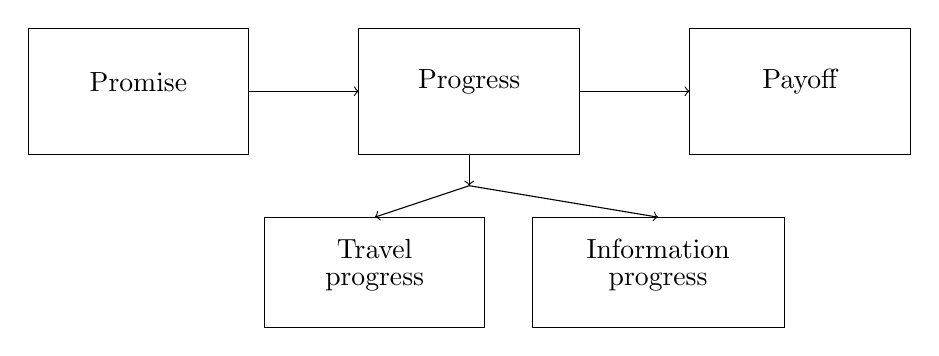
\begin{tikzpicture}
\draw (-5.2,0.8) rectangle (-2.4,-0.8);
\node at (-3.8,0.12) {Promise};

\draw (-1.0,0.8) rectangle (1.8,-0.8);
\node at (0.4,0.12) {Progress};

\draw (3.2,0.8) rectangle (6.0,-0.8);
\node at (4.6,0.12) {Payoff};

\draw[->] (-2.4,0) -- (-1.0,0);
\draw[->] (1.8,0) -- (3.2,0);

\draw (-2.2,-3.0) rectangle (0.6,-1.6);
\node at (-0.8,-2.0) {Travel};
\node at (-0.8,-2.42) {progress};

\draw (1.2,-3.0) rectangle (4.4,-1.6);
\node at (2.8,-2.0) {Information};
\node at (2.8,-2.42) {progress};

\draw[->] (0.4,-0.8) -- (0.4,-1.2);
\draw[->] (0.4,-1.2) -- (-0.8,-1.6);
\draw[->] (0.4,-1.2) -- (2.8,-1.6);
\end{tikzpicture}
\end{figure}

これは transcript-only の schematic である。lecture frames からの visual backing を claim するものではない。ただ、story の general structure と、progress が measured されうる different channels との distinction を display しているだけである。

彼の first example は geographic である。quest では、私たちは motion を space によって measure できる。

\begin{equation}
\text{travel progress} : \text{start} \to \text{destination}.
\end{equation}

lecture は careful であり、progress を constant な forward ease と equate しない。characters は diverted されるかもしれないし、backward へ forced されるかもしれないし、expected していた route から block されるかもしれない。だが、destination が stable enough であれば、その reversals は nonetheless legible である。``closer'' が何を mean するのかを define してくれるからだ。

second example は informational である。mystery では、progress は primarily spatial ではなく epistemic である。

\begin{equation}
\text{information progress} : \text{few clues} \to \text{more clues} \to \text{clearer picture}.
\end{equation}

したがって false clues や wrong turns も structure を destroy しない。reader が general image が sharpening しつつあると still feel できるなら、それらはむしろ structure に belong しているのである。

ここから Sanderson は pacing の diagnosis へ arrive する。story が slow に feel されるのは、nothing が occur していないからではなく、promised された kind of progress が clearly enough に signposted されていないからかもしれない。

\begin{equation}
\text{signposted progress} \Rightarrow \text{page-turning momentum}.
\end{equation}

そして converse も equally important である。

\begin{equation}
\text{misaligned signpost} \Rightarrow \text{perceived poor pacing}.
\end{equation}

\paragraph{Transcript note.} transcript は、この point の example において rough である。だが intended structural point は clear である。もし story が most strongly には adventure として signposted されているのに、writer が privately にはそれを romance として think しているなら、readers は progress を adventure axis に沿って measure することになる。そして promised されたその channel が advanced されていなければ、stasis を feel するだろう。

\subsection{Question \& Answer}

\paragraph{Question.} events が happening しているのに、なぜ story は slow に feel されるのか。

\paragraph{Answer.} events alone では momentum は generate されないからである。momentum には visible な progress channel が必要である。travel を promise したなら、reader は spatial advance を feel しなければならない。mystery を promise したなら、reader は accumulating information を feel しなければならない。その channel が weak であったり、story の strongest signposts と mismatch していたりすると、scenes が active であっても book は static に feel される。

Sanderson がこの section の within で与える final recommendation は practical で exact である。larger な progress channel を、smaller で legible な units、breadcrumb trail のようなものへ divide せよ、というのだ。そうすれば、reader は globally だけでなく locally にも motion を feel できる。

\section{mind を prime し、page より先に書く}

fifth で final の hack は、story の mechanics から work の mechanics へ return する。もし私たちが something like \(1{,}700\) words a day を aim しているなら、every session を cold に begin する afford はない。Sanderson の solution は、writing session そのものの before に mind を prime することである。

\begin{equation}
\text{off-page rehearsal} \to \text{on-page execution}.
\end{equation}

lecture は、この time がどの kinds のものを mean するのかについて concrete である。commuting、working out、doing dishes、mowing the lawn、body を occupy しつつ mind を comparatively free にしておく any activity である。その time を dissipate させる代わりに、次の scene が何を do すべきか、それを vivid にするものは何か、そしてなぜそれが book の memorable scenes の one になりうるのかを ask するために use できるのだ。

\paragraph{A worked routine.} Sanderson の method は、次のように summarize できる。
\begin{enumerate}
\item next に来る scene がどれかを decide する。
\item その scene の中で何が happen しなければならないかを ask する。
\item その scene を routine ではなく interesting にしているものは何かを ask する。
\item それを mentally に several times rehearse する。
\item next block of motion を already knowing した状態で sit down する。
\end{enumerate}

彼は even tonal refinement も add する。music が、scene の emotional register の中へ imagination を settle させる助けになることがあるのだ。point は ornament ではない。startup friction を reduce することにある。desk に reach するころには、scene は already mind の中で begin しているのである。

lecture はそのあと、この advice を one-month challenge の beyond へ generalize する。ordinary life が私たちに weekend writing time しか leave してくれないとしても、week の during に off-page priming を行えば、その later な hours を prepare できる。したがって lecture の final movement は structurally neat である。story を move させる方法を teach したあとで、Sanderson は writer 自身を move させ続ける方法を teach して close するのだ。

\section{まとめ}

この lecture は、casual な tone が first に suggest するより much more formal discipline をもって proceed する。私たちはまず numerical target と permission structure から begin する。quickly に write し、internal editor を turn off せよ。ただし、それが自分の psychology に against して work するなら、その challenge を worship するな、と。ついで私たちは outer structure を borrow し、monologue を通じて voice を discover し、wants と needs のあいだの tension から plot を generate し、story を promise、progress、payoff に compress し、そして最後に、page より先に think することによって whole enterprise を support する。

したがって、この chapter の central lesson は procedural である。novel は pressure の下で started されうる。ただし、その invention を十分な structure で stabilize するならである。external constraint、recoverable な pattern、character engine、visible な progress channel、そして intention と execution の gap を reduce する daily practice である。これが、Sanderson が私たちを lecture through に lead する order であり、notes が disconnected maxims の set ではなく unfolding する lecture のように feel されるのも、この order によるのである。